\chapter{Low-Power Firmware Design Techniques}

Chapter 5 gives a background on general sources of power consumption in a digital system and describes some of the primitive techniques used for power management. Section 5.4 describes the design flow of power management techniques for BlueBox system. Section 5.5 to 5.7 explains the details of those techniques.  
\section{Background} In order to design successfully for low power consumption, it is important to have a through understanding of the sources of power dissipation, the factors that affect them and the methodologies and techniques that are available to achieve optimal results. 
Throughout this chapter, we discuss about power consumption and methods for reducing it. Energy is the time integral of power; if power consumption is a constant, energy consumption is simply power multiplied by the time during which it is consumed. Reducing power consumption only saves energy if the time required to accomplish the task does not increase too much. The chapter presents the sources of power dissipation and describes the important low-power methodologies and power optimization techniques available. Low-power design can be applied on various abstracted levels, such as system level, architectural level and technological level. This chapter could as well be utilized as a quick review on low power design. 

\section{Sources of power consumption}\label{src_pwr}
Most components are currently fabricated using CMOS technology\cite{cypress, silicon}. Main reason for this bias is that CMOS technology is cost efficient and inherently lower power than other technologies. So the sources of power consumption talked in this chapter is based on CMOS component model. There are a number of sources of power consumption in CMOS, which can be subdivided into \textit{static} and \textit{dynamic} power dissipation. The main difference between them is that dynamic power is frequency dependent, while static is not. Dynamic power dissipation is primarily caused by the switching of the CMOS devices (MOSFETs) when logic values are changed (known as \textit{capacitive power} or \textit{switching power}). The amount of power that is dissipated is directly related to the switching activity (which is the number of logic transitions per clock cycle in the entire circuit), the clock frequency, the supply voltage, and the capacitive load the circuit drives \cite{PowerAwareDesign}. Another source of dynamic power dissipation is \textit{short-circuit power}. CMOS is comprised of both PMOS and NMOS devices. During a logic transition, the PMOS and NMOS devices are simultaneously turned on for a very short period of time, allowing a short-circuit current to run from V\textsubscript{dd} to ground\cite{Low-powercmos, LowPowerDesign}. This behavior is inherent to CMOS switching. The more dominant component of dynamic power is capacitive power. This component is the result of charging and discharging parasitic capacitances in the circuit. Every time a capacitive node switches from ground to V\textsubscript{dd} an vice-versa energy is consumed. 

 Static power, which is a constant factor and has nothing to do with the switching activity, is caused by \textit{leakage power}. In an ideal situation, a static CMOS circuit (i.e. one that does not switch) does not consume any power because there is no direct path from V\textsubscript{dd} to ground. In real life there will always be leakage currents, since CMOS devices are not perfect switches. The total power dissipation can be described by the following formula:
\[P_{total} = \alpha(C_L . V_{DD}^2.f_{clk}) + I_{sc}. V_{DD} + I_{leak} . V_{DD}    \hspace{10mm} (1) \]
\vspace*{-2mm}
The Greek letter $\alpha$ represents the \textit{switching activity} in the circuit, expressed in a value between 0 (no switching activity at all) to 1(maximum switching activity). C\textsubscript{L} is the capacitive load, driven by the circuit. As can been seen in the formula, the dynamic power consumption depends on V\textsubscript{dd} square, which makes the supply voltage a very important factor in low-power design, as will be explained later. I\textsubscript{SC} and I\textsubscript{leak} represent the total short circuit and leakage current, respectively. It is important to realize that that I\textsubscript{SC} is a variable, while I\textsubscript{leak} is not. I\textsubscript{SC} depends on the charge carried by the short-circuit per transition, the cycle time, and the total number of transitions
\vspace*{-2mm}
\[I_{SC} = Q_{SC}  \cdot  f \cdot \alpha    \hspace{10mm} (2) \] 
\vspace*{-2mm}
A better way to represent the formula would be like this:
\vspace*{-2mm}
\[P_{total} = \alpha(C_L \cdot V_{DD}^2 \cdot f_{clk}) +  Q_{SC}  \cdot  f_{clk} \cdot V_{DD} + I_{leak} \cdot V_{DD}    \hspace{10mm} (3) \]
 It is a misunderstanding that reducing power consumption will always lead to a reduction in energy as well. When we refer to power, we refer to the momentary electric energy that is dissipated, measured in Watts. Energy is measured in Joules, or Watts per second. Thus, the energy consumption depends on the power consumption and the time it takes to perform a task. For example, if we have two circuits A and B, and P\textsubscript{A} = 2P\textsubscript{B}, and 2D\textsubscript{A} = D\textsubscript{B} (where ’D’ refers to the delay of the circuits), then EA = EB. Thus, even though the power consumption of circuit B is twice as low as circuit A’s, no energy is saved. When we take another look at formula (3), reducing $\alpha$, V\textsubscript{DD}, and C\textsubscript{L} will always reduce power and energy consumption. Lowering f\textsubscript{clk} reduces
only power, not energy \cite{PowerAwareArchitecting}.

\section{Basic Low-Power Design Methodologies}
 The following methodologies are most powerful ones and are the most basic ones for any system. They include voltage scaling, frequency scaling, clock gating and power gating. All these methodologies helps to reduce the power consumption but comes at a cost. For example frequency scaling could affect the execution time of the application, power gating causes a boot up latency whenever the system or peripheral needs to be powered on. It purely depends on the application requirement to decide on the tradeoff. If the application can tolerate the cost of a methodology, then it can be used to reduce the power consumption. So, the BlueBox system adopts a few of these basic methodologies but not all of those. It is still important to have a basic idea of these basic methodologies and the insight they provide on power consumption. 
 
 \subsection{Static voltage scaling}
 One way to decrease the power consumption significantly, is to decrease the supply Voltage. As mentioned in the previous section \ref{src_pwr}, dynamic power consumption depends quadratically on V\textsubscript{DD}. Voltage scaling is therefore the most effective method to limit the power consumption. However, when V\textsubscript{DD} is lowered, it comes at a price: the delay of the logic 
 increases. In systems where we desire a high throughput, and ask for the maximum performance of the technology being utilized, voltage scaling is not an option. If V\textsubscript{DD} would be lowered, we would not be able to meet the performance requirements. In many 
 situations however, we do not ask for the maximum performance and we can safely lower V\textsubscript{DD} in order to save power. Even though delay is increasing, the power-delay product is improving when V\textsubscript{DD} is decreased, since power decreases quadratically while delay increases less fast. Delay scales with:
 \vspace*{-2mm}
 \[ \frac{V_{DD}}{
 	(V_{DD} - V_{TH})^2
 	} \hspace{20mm}(4)\]     
 
 \subsection{Dynamic voltage scaling}
 Instead of a fixed supply voltage during circuit operation it is also possible to dynamically 
 adjust the supply voltage based on the current required performance of the circuit. The required performance is often not always the same. When the required performance 
 of the circuit is momentarily reduced, we can afford lower supply voltages. This is called dynamic voltage scaling (DVS). Apart from lowering the supply 
 voltage, it is also possible to lower the clock frequency. A reduction in V\textsubscript{DD} will always 
 increase the delay to some extent, but if the cycle time is still much higher than the delay of the circuit, energy is wasted. Therefore dynamic voltage and frequency scaling (DVFS) can be employed to save energy to the maximum.
 
 \subsection{Frequency Scaling}
 Apart from V\textsubscript{DD}, there is another variable in the equation of section \ref{src_pwr} that intuitively 
 suggests possibilities for reducing power: frequency. Of course, the clock frequency is bound by the desired throughput of the system. However, a system does rarely operate at its maximum throughput all the time. Often, the desired throughput is much lower than its maximum performance. Then, it is possible to lower the operating frequency in order to save power (and thus also energy), which is called frequency scaling. Sometimes voltage scaling and frequency scaling are employed simultaneously, such as in cell phones, when they are in stand-by mode.
 
 \subsection{Clock gating}
 In the previous sections we have referred to (sub)systems that do not always operate at their maximum performance. It is also possible that parts of a system are idle for a 
 period of time: then no useful computational work is performed. Still, there is power consumed. A subsystem being idle does not necessarily mean that the subsystem is not performing any computations. It only means that the results are not being utilized. This is possible when the subsystem is still fed with data, but the result is discarded, because it is not needed at that moment. But even when the subsystem is not performing any computational work, there is still the static power dissipation (leakage power) of the subsystem. What is more, flip-flops dissipate some dynamic power every single clock cycle, even when the in- and outputs remain the same. If there are large registers present 
 in these subsystems, this power dissipation can become quite significant. And, finally, there is the power dissipation of the clock network in the subsystem. Clock networks are very expensive in terms of power. A major portion of the total power consumption of the system is dissipated in the clock network (mainly in the clock buffers/drivers) \cite{LowPowerMethod}. Considering the above, there is a lot of power that can be saved when a subsystem is idle. One way to achieve this goal is to apply clock gating. This essentially means that the clock signal of the subsystem is cut off. This will save the power dissipated in flip-flops and the clock network. If the combinational logic in the subsystem is fed by 
 registers at the inputs, the logic will stop switching \cite{DesignLowPower}. It will, however, not save the 
 leakage power.
 
 \subsection{Power Gating}
 Power gating provides basically a solution to the same problem mentioned in clock gating section. Power gating has however an important advantage over clock gating: it is capable to save static power of idle blocks as well, since it cuts of the power supply instead of 
 the clock signal. In order to do that, blocks need to be placed onto separate ”power domains”, which can be powered on and off. When a block is asleep it costs some time to wake it up again, the same as it costs 
 some time to put a block to sleep. This introduces additional delays. Also during wake-up and going to sleep, still some leakage power is dissipated which makes power gating not perfect. There is always a cost associated with the state transition. The essential criteria for implementing power gating is the total leakage power component and how many and how often blocks are idle. The leakage power highly depends on the technology being utilized and the impact of the leakage 
 power highly depends on the system frequency being utilized. If the leakage component is significant and many blocks are idle for longer periods of time, power gating may be efficient. One should however be aware of the fact that power gating is much more difficult to implement than clock gating and leads to significantly higher costs (mainly because of all the switches that are required). It is also important to realize that power 
 gating is much more invasive than clock gating. While clock gating does not affect the functionality of the system, power gating does. It affects inter-block communication and, as mentioned before, adds time delays to safely enter and exit power gated modes \cite{LowPowerMethod}. 
 
 \section{Design flow}
 
 Design flow of any system constitutes of various level of abstraction. Abstraction reduces complexity and allow efficient design and implementation of complex systems. The aspect of the system that needs to be optimized helps in designing the various levels of abstraction. When a system is designed with the emphasis on power optimization, then the design must embody optimization at all levels of the design flow. In general the support for energy management needs to be incorporated at the system level and the architectural level. An important aspect of the design flow is the relation and feedback between the levels. Paul J.M Havinga et. al, have come up with three layers of abstraction: system, architecture and technology \cite{havinga, havinga2, havinga3}. Table \ref{table:abstraction} describes the abstraction level and related examples for energy reduction.
 \begin{table}
 	\centering
 	\begin{tabular}{|l|l|}
 		\hline
 		Abstraction level & Examples  \\
 		\hline
 		  & processing method \\
 		  & energy manager \\
 		  System & scheduling \\
 		  & light weight filesystem \\
 		  & system partitioning \\
 		  & \\
 		  & parallel hardware \\
 		  Architecture & Direct Memory Access \\
 		  & FFT hardware \\
 		  &  \\
 		  & clock gating \\
 		  Technological & clock frequency control \\
 		  & voltage control \\
 		\hline
 	\end{tabular}
 	\caption{Abstraction level and related example for energy reduction.}
 	\label{table:abstraction}
 \end{table}


At the highest level the design decisions have the most influence. Therefore, the most effective design decisions derive from choosing and optimizing 
 architectures and algorithms at the highest levels. It has been demonstrated by several researchers [63] that system and architecture level design decisions can have dramatic impact on power consumption. However, when designing a system it is a problem to predict the consequences and effectiveness of high level design decisions because implementation details can only be accurately modeled or estimated at the technological 
 level and not at the higher levels of abstraction. Furthermore, the specific energy reduction techniques that are offered by the lower layers can be most effective only when the higher levels are aware of these techniques, know how to use them, and apply them.
 
 
The above mentioned layers can be considered as vertical layers of any digital system. The BlueBox system could be broken down into three main subsystem as shown in figure \ref{table:sub-system} based on its application semantics: sensor, processor and storage subsystem. These sub-systems work together and are interdependent on each other for their functionalities. Each of these subsystem contains all three abstraction layers mentioned above. Our low-power design flow targets each of these three horizontal layers of subsystem individually and the interdependent vertical layers within them. It is interesting that effect on a single subsystem creates space for further power savings for its dependent subsystem. 
 
  \begin{table}
 	\centering
 	\begin{tabular}{|l|l|}
 		\hline
 		$Sub$-$System$ & $Sub$-$System  components$  \\
 		\hline
 		& Accelerometer \\
 		& Environment Temperature sensor \\
 		Sensors & Audio Codec \\
 		& Ecg Analog Front end \\
 		& Body temperature sensor\\
 		\hline
 		& DSP core \\
 		Processor & GPIO \\
 		& Peripherals \\
 		& DMA \\
 		& Memory \\
 		\hline
 		Storage & SD card \\
 		& EMIF \\
 		\hline
 	\end{tabular}
 	\caption{Sub-Systems of BlueBox}
 	\label{table:sub-system}
 \end{table}
 
 
Our approach with this multi-dimensional design space offers us a large range of possible trade-offs. And our modeling of the system with horizontal and vertical layers made it fairly easy to think and work on power management. The following sections discusses our approach on minimizing power consumption in sensor, processor and storage subsystem.
 
 \section{Power Management of Sensor sub-system}
 
 A sensor is a device that converts real world physical parameters into electrical signals that a computer can understand. They are the most important active part of the BlueBox system. As shown in table \ref{table:sub-system} BlueBox employs five different sensors. Most of which are performing active real time sensing. They also do have a processing capabilities embodied with them. They contribute to the significant amount of power consumed by the system. The first, and perhaps most direct, approach of our low power consumption design targets the sensor itself. BlueBox employs power mode management, smart sensing and computational offloading techniques to reduce the power consumption of the DSP. The following section describes the three simple techniques that enabled low power sensing.
 \subsection{Sensor power mode management}
 Most of the sensors designed for low power consumption have one or more lower power states such as a shutdown mode or an extremely low-power operating mode \cite{lowpwrsensing}. In many instances, this types of sensor's operation is directly controlled by the firmware designer in the end application. It is also important to note that there is always a cost associated with the low power modes. The cost could be reduced performance, increased latency, delayed boot-up etc. And transition of modes consumes power too. So it is the application semantics that decides the best modes of operation and how often transition needs to be triggered. 
 
 
 Considering the body temperature sensor (MA100) from BlueBox system. It is eventually a thermistor. The voltage drop across this thermistor is a value proportional to the body temperature. The simplified circuitry of MA100 can be seen in figure \ref{body_temp}.
 \begin{figure}[h]
 	\centering
 	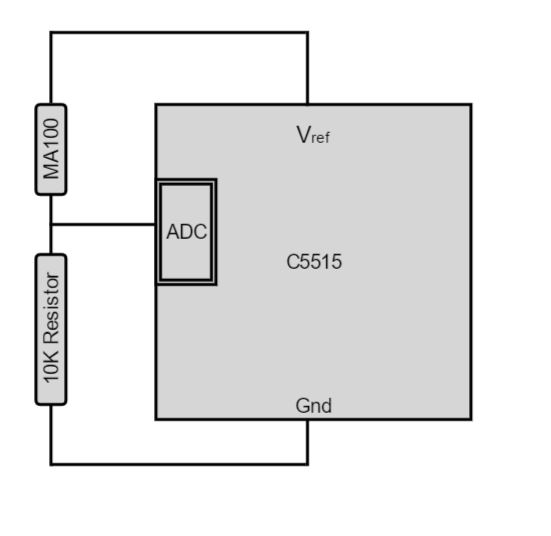
\includegraphics[scale = 0.5 ]{body_temp.JPG}
 	\caption{Simplified version Body Temperature measurement circuitry\label{body_temp}}
 \end{figure}
 The C5515 DSP supplies the reference voltage to the thermistor MA100. As body temperature is measured only twice in a second, the reference voltage could be supplied only during the measurement and can be turned off the rest of the time to save the power dissipated by the measurement circuit during the unused time.
 
From \ref{mpu9250_def} it can be noticed that the Accelerometer sensor(MPU9250) takes 30ms to wakeup from sleep and generate a valid accelerometer value. BlueBox cannot afford to spend this time inside the ISR. So it is a good idea to keep the MPU9250 under low-power accelerometer mode, which consumes 19.8 $\mu$A providing the required response time.
 
 \subsection{Smart Sensing}
 Smart sensing is a method for achieving low power that uses integrated 'smart' digital logic in the sensor. "Smart Sensing" is the added digital capability which can be used to enable the sensor to perform its own internal power management or help reduce the power consumption of the system. This approach has been used in BlueBox through the smart capabilities of accelerometer.
 
 The sensor's embedded logic detects events and notifies the DSP over interrupt. Unlike the previous low-power method that has no power consumption at its lowest level, this one has a baseline power consumption, so it can automatically power itself on. With a higher frequency of use, a device with more internal intelligence eventually becomes more efficient. 
 
An example of such technique in the BlueBox, for reducing power consumption is the use of accelerometer’s smart first in, first out (FIFO) buffer. An 8-bit or 12-bit configurable 32-sample FIFO allows buffering of the data so a host system can power on the sensor and read the data at a slower rate. As a result, the DSP can be kept in a lower power state more of 
 the time, achieving lower power consumption for itself and lower duty cycle operation for the DSP whose power consumption is approximately ten times higher than the accelerometer’s power consumption. By reducing the DSP’s power on time by a very small amount, the entire system might still consumes less power even though the accelerometer consumes more power. The system-level advantages more than compensate for the slightly 
 higher power consumption in the sensor. 
 
 \subsection{Computational offloading}
 In this third approach for low power sensing, the DSP utilizes the local computing capability of the sensor. Termed "local compute capability", this system level methodology can offload the computation from system application DSP. For example, a DSP that uses 100 to 1000 times as much power, a local sensor with the compute capability can perform the required computations and allow the DSP to go into lower power modes delivers a significant power savings at the system level, resulting in savings.  
 
  \begin{figure}[h]
 	\centering
 	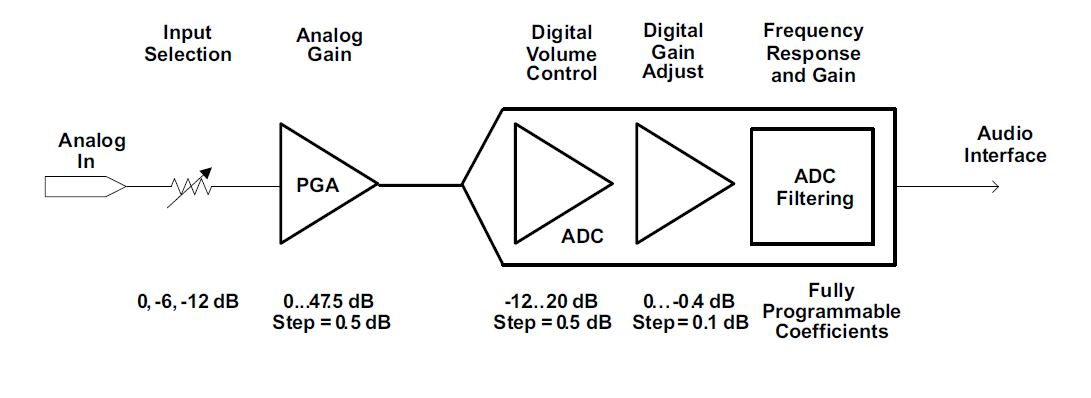
\includegraphics[scale = 0.5 ]{AIC_processingBlock.JPG}
 	\caption{Signal Processing blocks of Audio Codec. \cite{audiocodec} \label{AIC_processingBlock}}
 \end{figure}
 
This design methodology is used in BlueBox to reduce the power consumption of audio data acquisition through the use of local compute capability of the Audio Codec. Audio signal captured through the electret microphones contains some noise with it. And is required to filter the signal to improve the audio quality and attenuate high frequency noises. The process of digital filtering at the DSP could be a good solution as the filter can be designed specific for the application and the signal of interest. But it consumes lots of computational bandwidth and power which is not very desirable for the BlueBox application. So BlueBox uses the signal processing support extended by the audio codec AIC3204 as shown in figure \ref{AIC_processingBlock}. The codec has a fixed number of filters with configurable coefficients. So this application specific filtering circuits in the codec would be more efficient, perform faster and consume significantly less energy than doing the same filtering process in the general purpose processor. Offloading the digital filtering computation to the codec saves a significant amount of computational bandwidth and power.
 
\section{Power Management of DSP subsystem }

Selecting a processor is one of the most critical decisions when we are designing an embedded 
system. This selection is based on the features required to satisfy the control functionality of the final product and the raw computing power needed to fulfill those system requirements. There are several points to be aware of when selecting a processor. The overall power consumption of a MCU is defined by its power consumption in different modes, typically active and standby (including sleep, idle, standby, etc.), and taking into account the power consumed to transition from one mode to another. 

 Active power consumption by a processor is the power consumed when the processor is running. As almost all controllers are based upon CMOS logic, power is consumed primarily during the switching of transistors. The other major factor which determines the run time of the system is the standby power consumption. Most applications can spend significant amount of time in standby mode. Standby current is the sum of leakage current, current consumed by power management circuits, clocking systems, power regulators, RTC, IOs, interrupt controllers, and so on. It varies from controller to controller, based upon the particular features and peripherals supported in standby mode. The power consumed in standby mode is significantly very less than in active mode. So the basic idea is to put the processor into standby mode when ever it is possible and try to keep the processor idle as long as possible to reduce the power consumed by the processor. The following section discusses the techniques used in the BlueBox system to reduce the processor power consumption. 


 Timing analysis is the first step towards the understanding of the processor functionality in terms of processor utilization \cite{sastra}. The processor utilization 'U' is defined as the total amount of time spent idle by the processor. 
\[ U = 100\% - (\% T_{idle}) \hspace{20mm} (1)\]

 Idle time is the time during which processor does not do any useful work. Normally this is an infinite loop that spins the processor waiting for an event. The code composer studio IDE, which is used for firmware development, provides the timing analysis of the code execution in DSP. Once the average idle time is known, we can measure the active utilization when the system is under various states of loads using the equation (1). BlueBox employs Intelligent waiting, even reduction and intelligent peripheral shutdown techniques to reduce the power consumption of the DSP. The following sections explains each of the technique in detail. 

\subsection{Intelligent Waiting}
The TMS320C5515 DSP includes various run-time power modes that can be used to scale down power consumption. The most common of important is idle mode of operation, in which the instruction-executing portion of the processor core shuts down while all peripherals and interrupts remain powered and active. Idle mode consumes substantially less power than the processor is actively executing instructions. A key aspect of idle mode is that it requires little overhead to enter and exit, usually allowing it to be applied many times every millisecond. Anytime the DSP is spinning in a loop or blocked waiting for an event it should be placed into idle mode to conserve power. Since any interrupt can wake the DSP from idle mode, use of this mode enables the DSP to intelligently wait for events in the system. The BlueBox system is dependent on external interrupts generated by the ECG analog frontend and the audio codec through the I2S bus. From figure \ref{main} it can be seen that the main thread of the BlueBox goes to idle mode after writing the pages to SD card, if they are available. When an interrupt occurs, the DSP wakes up and interrupt is serviced. Then the DSP checks if any page is available to write and then goes back into the idle mode to save power. 


\subsection{Event reduction}
Another important technique employed is the event reduction. Intelligent waiting enables the processor to enter its idle mode as often as possible, event reduction attempts to keep the processor in idle mode as long as possible. It is implemented by analyzing the application firmware code and system requirements to determine the effect of alteration of processing the interrupts. The interrupts associated with the BlueBox are periodic external interrupts that informs the processor to read an collect the data. There are totally 24000 audio interrupts generated every second by the audio codec. If the processor handles all the interrupts, it will not have suffient time to go to idle mode and have to be active all the time. This is where Direct Memory Access(DMA) comes into play to help the processor. Direct memory access (DMA) allows the processor to remain in idle mode for significant periods even while data is being sent to 
or received from peripherals. DMA should be used in peripheral drivers whenever possible. The savings are quite impressive. The DMA employed with the audio codec reduces 24000 interrupts per second to 24 interrupt per second. Figure \ref{event_reduction} explains how the reduction is achieved.
 \begin{figure}[h]
	\centering
	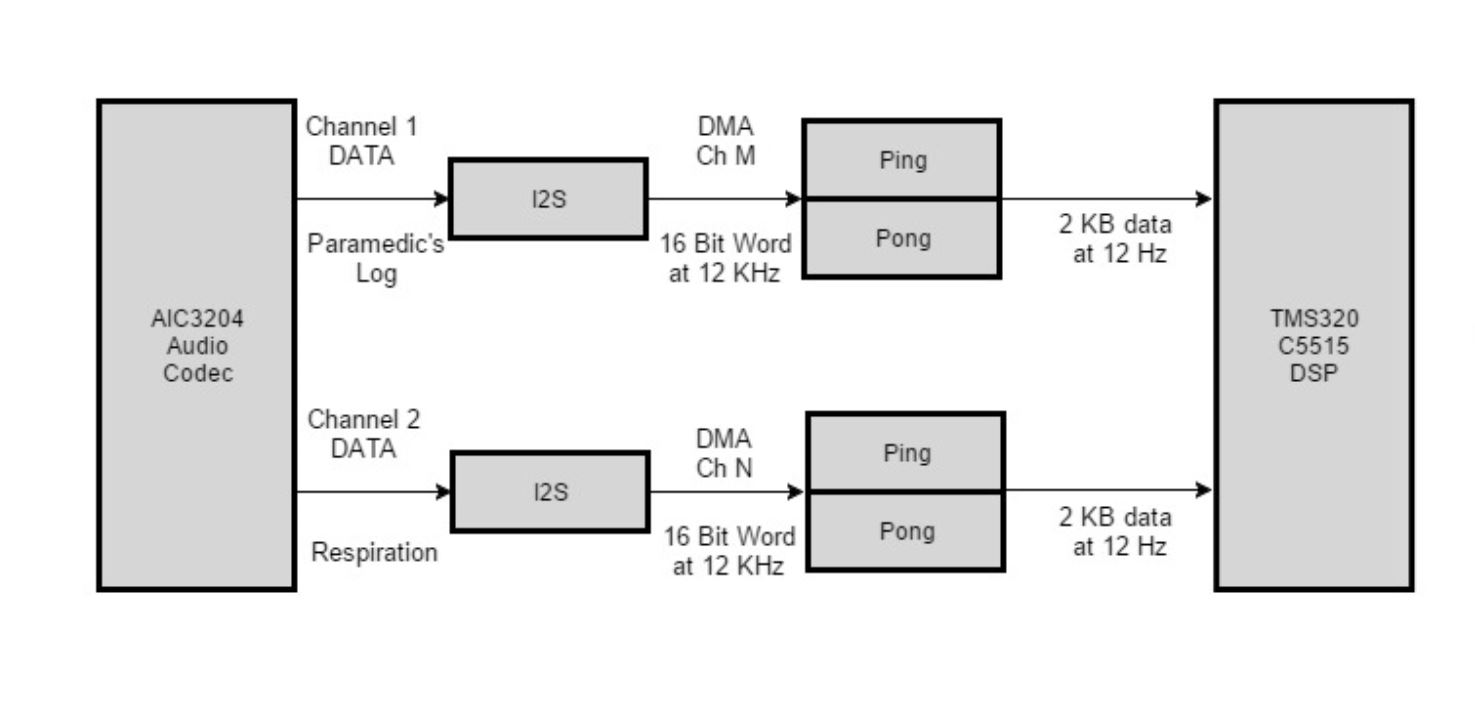
\includegraphics[scale = 0.5 ]{Event_Reduction.JPG}
	\caption{Event Reduction through DMA for Audio acquisition\label{event_reduction}}
\end{figure}


 The receiver DMA ping-pong buffer is of 2KB size and it takes 1000 interrupts and move the data into the buffer. When the buffer is full, the DMA interrupts the processor to take further actions. In the mean time the DMA starts servicing the interrupts filling up the pong buffer. Therefore during the situations where the processor is more prone to face the external interrupts, the event reduction approach using the DMA will be the solution.
 
 The intelligent waiting and the event reduction techniques together has brought down the DSP active time, utilization, to roughly 20.92 \%. The details of the calculation are presented in section \ref{utilization_result}.

\subsection{Intelligent peripheral shutdown}
All the above methods are for the power consumption when the device is running. This method of intelligent shutdown is useful when the peripheral is clock or power gated when it is not in use. The C5515 processor continues to power the general purpose input output pins and peripherals during idle mode. As inputs, these I/O pins can be used as interrupts to wake up the device; as outputs, they can be used to configure to external peripherals. Careful configuration of how these pins are configured can have large effect on sleep mode power consumption. The DSP has separate power domains which provide power to different portions of the device. The separate power domains allows the firmware to select the optimal voltage to achieve the lowest power consumption at the best possible performance. There are 13 different power domains each of which powers a specific domain. Figure \ref{power_domain} gives the brief gist of the power domains. Body temperature is measured twice in a second. From figure \ref{body_temp} shows the simplified body temperature measurement circuitry. It can be understood that the ADC peripheral of the DSP will be used only twice every second. So BlueBox firmware enables the Analog power domain that powers the ADC only during the measurement. The Analog power domain and also the ADC peripheral is shutdown during the rest of the time. 

\section{Power management of Storage Subsystem}
Storage contributes to a significant fraction of power consumption of embedded system. With respect to data acquisition and logging system the fraction is somewhere between 30 to 50 \% . From the table \ref{table:power_rating} we can notice that power consumption of SDHC card is approximately equal to 50\% of the entire system when a read or write action is performed. It is thus required to manage the storage sub-sytem with atmost care. So the basic idea is to write or read as minimum as possible and only when it is required and keep the SDHC card utilization as low as possible.
Storage subsystem involves the SDHC card and MMCSD interface from the DSP. As mentioned in section \ref{memory} SDHC card is block addressable. Blocks of size 512 bytes can be written or read from the SD card. So the processor has to buffer or cache blocks of data and write them into the SD card.  

The five different signals have to be stored in the SD card. BlueBox system groups these signals into two category. One just has the audio signal and other has ECG, accelerometer and temperature data. There are buffers associated with each of these categories and the respective data is written into them and eventually flushed to the SD card. The reason for such categorization is because of the amount of data produced by these signals. Audio data is produces at a rate of 48 kilobyte every second, so it makes sense to have dedicated buffer for themselves to be stored. The other signals are sampled comparatively very less, so they could be grouped together to share buffers and are written into the SD card. 

 The ECG analog front end interrupts the DSP at a frequency of 500Hz. Each sample collected during the interrupt is appended to the buffer. Because accelerometer only needs to be sampled at 12Hz, a counter within the interrupt ensures that accelerometer is sampled only once every 40 interrupts. Similarly the temperature is to be sampled at 2 Hz, a counter within the interrupt service routine is used to make sure samples are taken every 250 interrupts. Each time the signals are sampled, values from each of the sensors are stored in the respective position in the buffer. 
\subsection{Saving data to micro SD card}

Because the BlueBox must be able to function continuously, the interrupt services must continue to operate even when data is being written to SD card. So DMA's are used to write the data into the SD card as it can do the task without the interference of the DSP. When possible, sampled data is saved directly to a primary data buffer. When the primary data buffer is full DMA is instructed to initiate the transfer of the data from primary buffer into the SD card persistent storage. In the meantime data collected is stored in the secondary buffer and the cycle goes on. 

 There are lot of different ways of writing and organizing the data in the SD card. One way is to use existing filesystem that is recognizable by the general operating system, other way is to write the raw data and to design a n application specific custom filesystem. There are pros and cons associated with designing a new filesystem. Using a existing standard filesystem like FAT, NTFS etc., are really simple to implement as standard libraries are present but they were all designed for user comfortability and are designed for higher end computational devices. There is a huge overhead associated with storing and reading of data. For example, in order to write a block of data into a file, first it takes multiple SD card reads to figure out to which block address the data should be written then the actual processes of writing happens. This process keeps the SD card busy for longer duration, which is very undesirable for our application. It is required to come up with a simple custom filesystem that could suffice the necessity of application. The problems of custom filesystem is incompatibility with standard operating systems. To read data from the custom formatted SD card, it is required to develop a filesystem driver which is capable of reading this SD card. It requires some time to implement and test the custom filesystem. The important thing here to notice is that the custom filesystem could potentially save time and power it consumes to write data to the SD card.


\subsection{File System}\label{filesystem} 

A Secure Digital High Capacity(SD) card basically has a SD controller module and a memory core. Memory core is where the data is stored in. The memory core of a SDHC card is divided into blocks of 512 bytes and they are block addressable. BlueBox caches the data in a local buffer, which are, in general multiples of block size of the SD card. For convenience of understanding, the buffer that caches the data is referred as pages. The custom filesystem developed for bluebox has three categories of pages. They are audio page(same page layout used for both the channels of audio), vitals page(includes ECG, temperature and accelerometer data) and index page. The page size used for audio is 2Kb and for ECG its 512 bytes.
 Figure \ref{audio_page} shows the layout of audio page. It just contains the actual audio data and does not encode any meta-data with it. The pointers to the audio pages are present in the Index page. Each audio page accounts for four blocks, so when ever an audio page is written to the SD card, the corresponding four block address are stored in the index page. 
\begin{figure}[h]
	\centering
	\hspace*{-2cm} 
	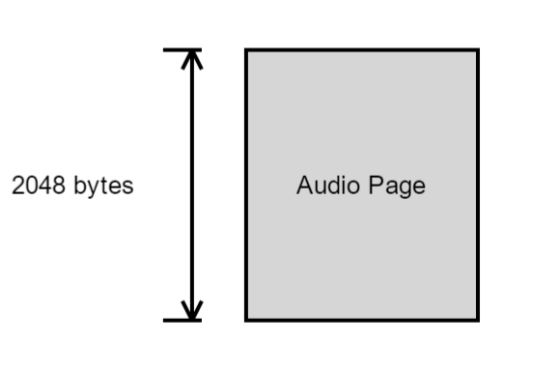
\includegraphics[scale = 0.5 ]{audio_page.JPG}
	\caption{Audio Page\label{audio_page}}
\end{figure}

\begin{figure}[h]
	\centering
	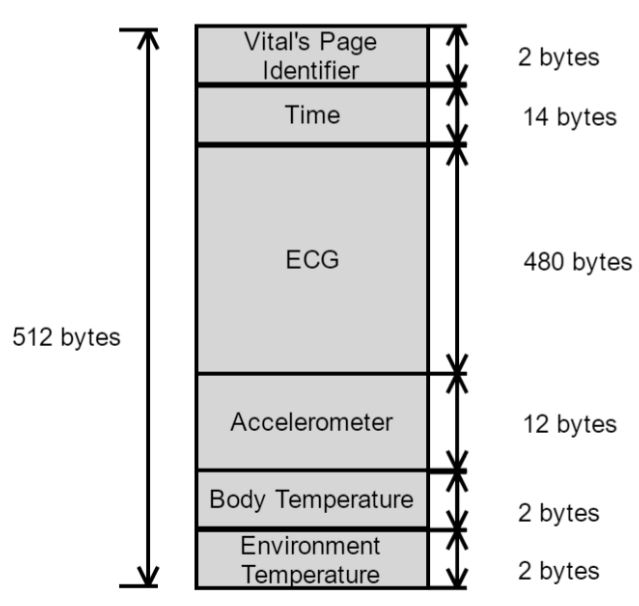
\includegraphics[scale = 0.5 ]{vital_page.JPG}
	\caption{Vitals Page\label{vital_page}}
\end{figure}


Figure \ref{vital_page} depicts the Vitals page. Its 512 bytes in size and contains actual data along with meta data. The first two bytes of the vitals page is an identifier, which uniquely identifies it. It includes ECG, accelerometer, temperature and time data. 


 The index page comprises of a 2 byte page identifier, 2 byte Audio channel identifier and 127 32bit block address as shown in figure \ref{index_page}. There is a separate index pages for left and right channel audio. The block addresses in the index pages are the pointers to next pieces of the audio data. The audio data is reconstructed into a file using these index pages.
 
\begin{figure}[h]
	\centering
	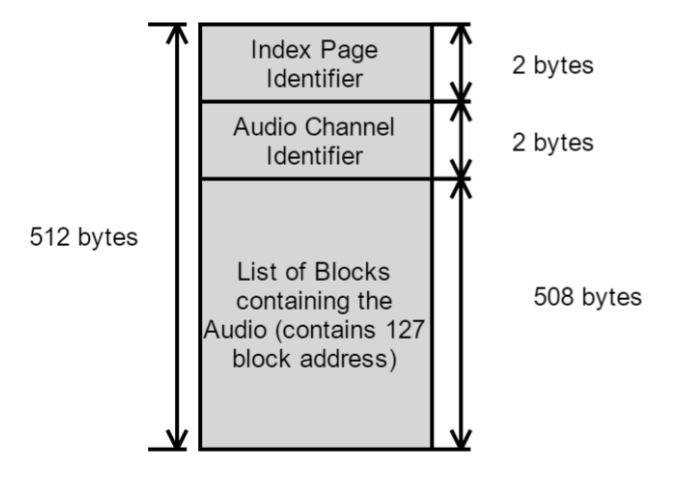
\includegraphics[scale = 0.5 ]{index_page.JPG}
	\caption{Index Page\label{index_page}}
\end{figure}

 The firmware filesystem driver keeps track of the next available free block and decides to which block does the data in the page go into. All the pages are written to the SD card sequentially. After the page has been successfully written by the DMA, the block address pointer is updated to point to the next free block. 24 pages of audio sample is written per second and 4 pages of ECG and other aggregated data is written per second. The filesystem inherently keeps track of content of each block through page identifiers and the pointers in the index page. The index page is also cached in a buffer and when it fills up it is written into the SD card. So that while reading back the data from the SD card we could organize the blocks and reconstruct the data stream.  

 This simple custom filesystem helped in reducing the overhead of writing data to SD card, which in general is very high with a standard filesystem that adds up bunch of meta data. The following graph \ref{fig:fs_time} shows the time taken to write the data to sd card and compares the two filesystem. The x axis marks the amount of data( includes only the meaningful sensor data) and the y axis marks time in millisecond.
{
\centering
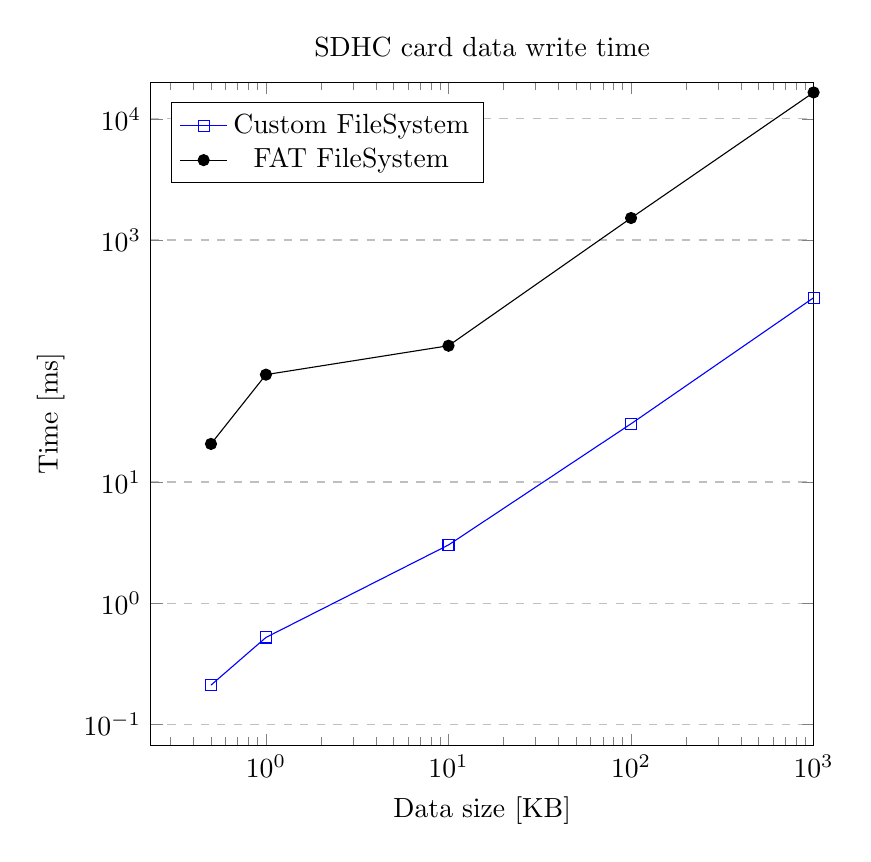
\begin{tikzpicture}
\begin{axis}[
title={SDHC card data write time},
xmode=log,
ymode=log,
height =100mm,
width = 100mm,
xlabel={ Data size [KB]},
ylabel={Time [ms] },
xmin=0, xmax=1000,
ymin=0, ymax=20000,
xtick={0.1,1,10,100,1000},
ytick={0.1,1,10,1000,10000,100000},
legend pos=north west,
ymajorgrids=true,
grid style=dashed,
]

\addplot[
color=blue,
mark=square,
]
coordinates {
	(0.5,0.21)(1,0.52)(10,3.02)(100,30.28)(1000,333.09)
	
};
\addlegendentry{Custom FileSystem}

\addplot[
color=black,
mark=*,
]
coordinates {
	(0.5,20.644)(1,77.15)(10,133.70)(100,1517.986)(1000,16552.70)
	
};
\addlegendentry{FAT FileSystem}

\end{axis}
\end{tikzpicture}\label{fig:fs_time}

}

 From the figure \ref{fig:fs_time} it is evident that for the same amount of actual data the custom filesystem takes, on an average, 50x less time to write than the FAT filesystem. The custom filesystem essentially spends less energy to save the data by reducing the active utilization time by 50x. 

From the experiment with SDHC card, running at 20MHz clock at 3.3 V, the write/read operation consumes 48 mA (considering only DSP and SD card active) and in standby it consumes 22 mA. BlueBox system requries to write 50 KB of data every second as mentioned in section \ref{system requirements}. The utilization of storage(U\textsubscript{storage}) using the custom filesystem can be computed as follows:
 \[U_{storage} = \frac{Time taken to store 50 KB}{
	F_{DSP}
} * 100 \%\]

 \[U_{storage} = \frac{1,514,088}{
	100,000,000
} * 100 \% = 1.5\%\]

 With FAT filesystem, the storage utilization is closer to 70\% whereas it is just 1.5\% with the custom file system.
 The system draws an average current of 40.2 mA when writing 50KB of data in one second on FAT filesystem whereas the custom filesystem's average current consumption is 22.27 mA. Thus the designed filesystem reduces the system's average power consumption by approximately 44.6\% within the application semantics of BlueBox. 
 
\nomenclature{DVFS}{ Dynamic Voltage and Frequency Scaling }
\nomenclature{GPIO}{ General Purpose Input Output }
\nomenclature{MCU}{ Micro controller Unit }
\nomenclature{FAT}{ File Allocation Table }
\nomenclature{NTFS}{ New Technology File System }  